\documentclass[12pt]{article}
\usepackage{amssymb, amsmath}
\usepackage{graphicx,tikz}
\usepackage{fancyhdr}
\usepackage{enumerate} 
\setlength{\headheight}{28pt}
\usepackage[top=1.0in, bottom=0.5in, left=0.75in, right=2.5in]{geometry}
\pagestyle{fancy}
\fancyhf{}
\lhead{MATH3004 HW \#0\\ Fall 2017}
\rhead{\thepage}
\chead{Rob Ireton}

\title{Homework 0}
\newcommand{\zee}{\mathbb{Z}}

\begin{document}

This assignment is just to make sure that you are able to type up and submit your work using latex.

Make sure you put your name in the header above.

Please make a typed version of the statement below, making it have the same formatting to the best of your ability.

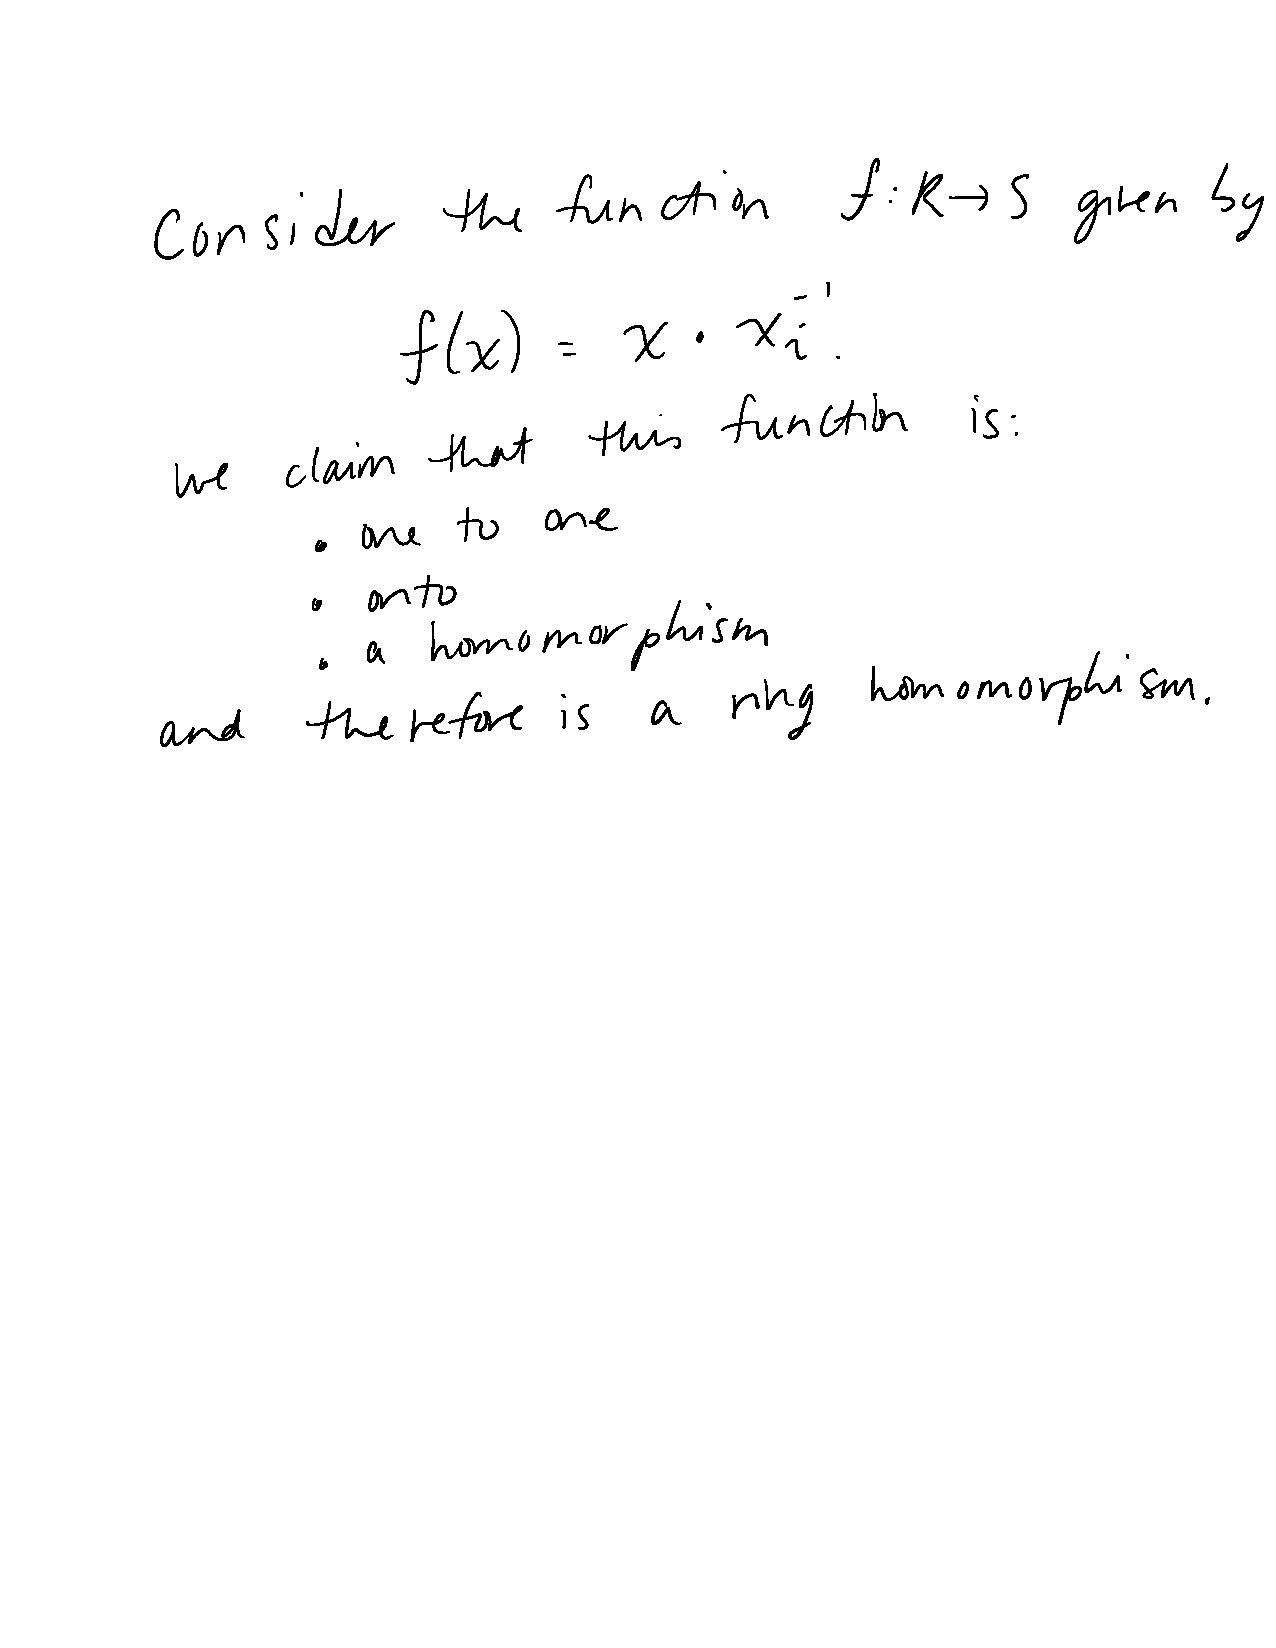
\includegraphics[width=\textwidth]{hw0ex}

Consider the function \(f: \mathbb{R} \to S\) given by
\[ f(x) = x \cdot x_i^{-1}\]
We claim that this function is:
\begin{itemize}
\item one to one
\item onto
\item a homomorphism
\end{itemize}
and therefore is a ring homomorphism.

\end{document}


